\documentclass[aspectratio=169, 10pt]{beamer}
\usetheme{metropolis}

\usepackage{pgfplots}
\pgfplotsset{compat=1.18}
\usepackage{tikz}
\usetikzlibrary{arrows.meta, positioning, shapes.geometric, fit, backgrounds, decorations.pathreplacing}
\usepackage{booktabs}
\usepackage{xcolor}
\usepackage{amsmath}

% ── Colour palette ────────────────────────────────────────────────────────────
\definecolor{NavyBlue}{HTML}{1B3A5C}
\definecolor{SteelBlue}{HTML}{2E75B6}
\definecolor{LightBlue}{HTML}{BDD7EE}
\definecolor{Amber}{HTML}{E67E22}
\definecolor{Green}{HTML}{27AE60}
\definecolor{LightGray}{HTML}{F5F5F5}
\definecolor{MidGray}{HTML}{7F7F7F}
\definecolor{CPURed}{HTML}{C0392B}
\definecolor{GPUBlue}{HTML}{2980B9}

% ── Metropolis overrides ───────────────────────────────────────────────────────
\setbeamercolor{normal text}{fg=NavyBlue, bg=white}
\setbeamercolor{frametitle}{bg=NavyBlue, fg=white}
\setbeamercolor{title separator}{fg=SteelBlue}
\setbeamercolor{progress bar}{fg=SteelBlue, bg=NavyBlue!20}
\setbeamercolor{alerted text}{fg=Amber}
\setbeamercolor{block title}{bg=SteelBlue!15, fg=NavyBlue}
\setbeamercolor{block body}{bg=LightGray}
\setbeamerfont{frametitle}{size=\large, series=\bfseries}
\setbeamerfont{title}{size=\LARGE, series=\bfseries}
\setbeamerfont{subtitle}{size=\normalsize}

% ── Metadata ──────────────────────────────────────────────────────────────────
\title{RFdiffusion Inference Optimization}
\subtitle{Dry Lab Progress Update}
\institute{iGEM Team}
\date{\today}

% ── Helper: section divider ───────────────────────────────────────────────────
\newcommand{\sectionslide}[1]{%
  \begin{frame}[plain]
    \begin{tikzpicture}[remember picture, overlay]
      \fill[NavyBlue] (current page.south west) rectangle (current page.north east);
      \node[white, font=\LARGE\bfseries, align=center] at (current page.center) {#1};
    \end{tikzpicture}
  \end{frame}
}

\begin{document}

% ══════════════════════════════════════════════════════════════════════════════
%  TITLE
% ══════════════════════════════════════════════════════════════════════════════
\begin{frame}[plain]
\begin{tikzpicture}[remember picture, overlay]
  % Background
  \fill[NavyBlue] (current page.south west) rectangle (current page.north east);
  % Accent bar
  \fill[SteelBlue] ([yshift=-0.35\paperheight]current page.north west)
    rectangle ([yshift=-0.40\paperheight]current page.north east);
  % Title
  \node[white, font=\LARGE\bfseries, align=left, anchor=west]
    at ([xshift=1cm, yshift=0.12\paperheight]current page.west)
    {RFdiffusion Inference Optimization};
  % Subtitle
  \node[LightBlue, font=\large, align=left, anchor=west]
    at ([xshift=1cm, yshift=0.04\paperheight]current page.west)
    {Dry Lab Progress Update};
  % Institute
  \node[white!70!NavyBlue, font=\normalsize, align=left, anchor=west]
    at ([xshift=1cm, yshift=-0.04\paperheight]current page.west)
    {iGEM Team};
  % Date
  \node[white!60!NavyBlue, font=\small, anchor=south east]
    at ([xshift=-1cm, yshift=0.5cm]current page.south east)
    {\today};
\end{tikzpicture}
\end{frame}

% ══════════════════════════════════════════════════════════════════════════════
%  AGENDA
% ══════════════════════════════════════════════════════════════════════════════
\begin{frame}{Agenda}
\begin{tikzpicture}
  \foreach \i/\label/\col in {
    1/{Project Context}/NavyBlue,
    2/{Problem Identification}/NavyBlue,
    3/{Root Cause Analysis}/NavyBlue,
    4/{Solutions Implemented}/NavyBlue,
    5/{Results}/NavyBlue,
    6/{Hardware Landscape}/NavyBlue,
    7/{Future Work}/NavyBlue
  }{
    \node[draw=\col, fill=\col!8, rounded corners=3pt,
          text width=3.2cm, align=center, minimum height=1cm,
          font=\small\bfseries, text=\col]
      at ({(\i-1)*2.1cm}, 0) {\label};
    \ifnum\i<7
      \draw[-{Stealth[scale=0.8]}, \col!50, thick]
        ({(\i-0.5)*2.1cm - 0.3cm}, 0) -- ({(\i-0.5)*2.1cm + 0.3cm}, 0);
    \fi
  }
\end{tikzpicture}
\end{frame}

% ══════════════════════════════════════════════════════════════════════════════
%  1. PROJECT CONTEXT
% ══════════════════════════════════════════════════════════════════════════════
\sectionslide{1. Project Context}

\begin{frame}{RFantibody is Central to Our Design Pipeline}
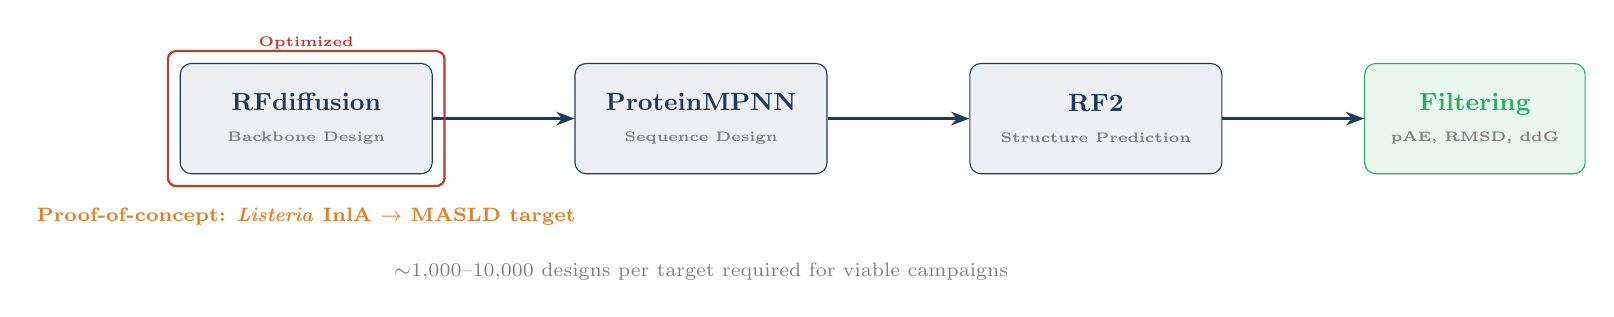
\begin{tikzpicture}
  % Pipeline boxes
  \node[draw=NavyBlue, fill=NavyBlue!8, rounded corners=4pt,
        minimum width=3.2cm, minimum height=1.4cm, align=center,
        font=\small\bfseries, text=NavyBlue] (diff) at (0,0)
    {RFdiffusion\\{\tiny\color{MidGray}Backbone Design}};

  \node[draw=NavyBlue, fill=NavyBlue!8, rounded corners=4pt,
        minimum width=3.2cm, minimum height=1.4cm, align=center,
        font=\small\bfseries, text=NavyBlue, right=1.8cm of diff] (mpnn)
    {ProteinMPNN\\{\tiny\color{MidGray}Sequence Design}};

  \node[draw=NavyBlue, fill=NavyBlue!8, rounded corners=4pt,
        minimum width=3.2cm, minimum height=1.4cm, align=center,
        font=\small\bfseries, text=NavyBlue, right=1.8cm of mpnn] (rf2)
    {RF2\\{\tiny\color{MidGray}Structure Prediction}};

  \node[draw=Green, fill=Green!10, rounded corners=4pt,
        minimum width=2.8cm, minimum height=1.4cm, align=center,
        font=\small\bfseries, text=Green, right=1.8cm of rf2] (filter)
    {Filtering\\{\tiny\color{MidGray}pAE, RMSD, ddG}};

  % Arrows
  \draw[-{Stealth}, NavyBlue, thick] (diff.east) -- (mpnn.west);
  \draw[-{Stealth}, NavyBlue, thick] (mpnn.east) -- (rf2.west);
  \draw[-{Stealth}, NavyBlue, thick] (rf2.east) -- (filter.west);

  % Optimization label
  \draw[CPURed, thick, rounded corners=3pt]
    ([xshift=-0.15cm, yshift=0.15cm]diff.north west) rectangle
    ([xshift=0.15cm, yshift=-0.15cm]diff.south east);
  \node[CPURed, font=\tiny\bfseries, above=0.05cm of diff] {Optimized};

  % Scale annotation
  \node[MidGray, font=\scriptsize, align=center, below=1.0cm of mpnn]
    {$\sim$1{,}000--10{,}000 designs per target required for viable campaigns};

  % PoC annotation
  \node[Amber, font=\scriptsize\bfseries, align=center, below=0.3cm of diff]
    {Proof-of-concept: \textit{Listeria} InlA $\rightarrow$ MASLD target};
\end{tikzpicture}
\end{frame}

% ══════════════════════════════════════════════════════════════════════════════
%  2. PROBLEM IDENTIFICATION
% ══════════════════════════════════════════════════════════════════════════════
\sectionslide{2. Problem Identification}

\begin{frame}{The A100 Server Was Slower Than a Desktop GPU}
\begin{columns}[c]
\begin{column}{0.55\textwidth}
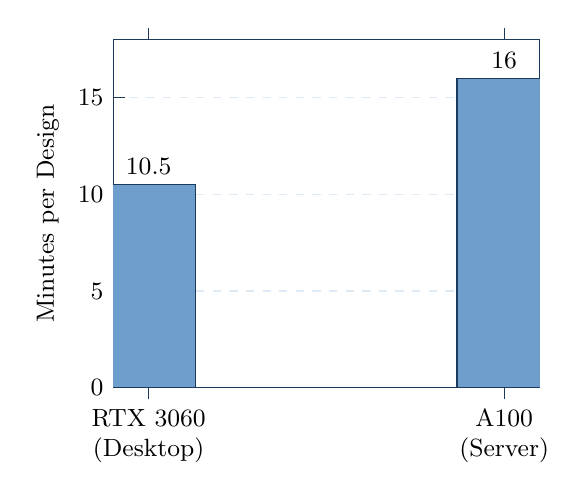
\begin{tikzpicture}
\begin{axis}[
  ybar,
  bar width=1.2cm,
  width=7cm, height=6cm,
  ymin=0, ymax=18,
  ylabel={Minutes per Design},
  ylabel style={font=\small},
  symbolic x coords={RTX 3060\\(Desktop), A100\\(Server)},
  xtick=data,
  xticklabel style={align=center, font=\small},
  ytick={0,5,10,15},
  yticklabel style={font=\small},
  axis line style={NavyBlue},
  tick style={NavyBlue},
  ymajorgrids=true,
  grid style={dashed, LightBlue!50},
  nodes near coords,
  nodes near coords style={font=\small\bfseries},
]
\addplot[fill=SteelBlue!70, draw=NavyBlue] coordinates {
  ({RTX 3060\\(Desktop)}, 10.5)
  ({A100\\(Server)}, 16)
};
\end{axis}
\end{tikzpicture}
\end{column}
\begin{column}{0.42\textwidth}
  \begin{block}{The Paradox}
    \small
    The A100 has \textbf{6$\times$ the compute} of an RTX 3060, yet was \textbf{50\% slower} per design.
  \end{block}
  \vspace{0.4cm}
  \begin{alertblock}{At 1{,}000 Designs}
    \small
    \textbf{A100:} $\sim$267 hours\\
    \textbf{RTX 3060:} $\sim$175 hours\\[0.3em]
    The expensive server was the wrong choice.
  \end{alertblock}
\end{column}
\end{columns}
\end{frame}

% ══════════════════════════════════════════════════════════════════════════════
%  3. ROOT CAUSE ANALYSIS
% ══════════════════════════════════════════════════════════════════════════════
\sectionslide{3. Root Cause Analysis}

\begin{frame}{Each Diffusion Timestep Repeatedly Stalled the GPU}
\begin{center}
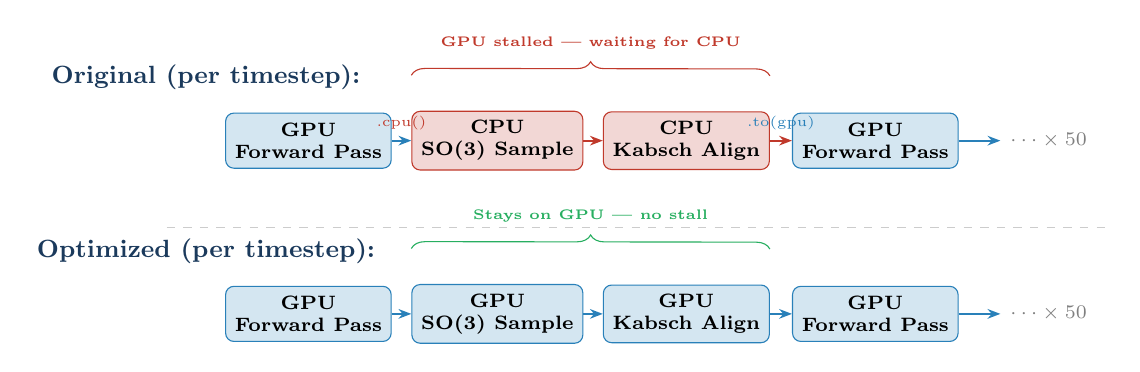
\begin{tikzpicture}[
  box/.style={rounded corners=3pt, minimum width=2.0cm, minimum height=0.7cm,
              align=center, font=\scriptsize\bfseries},
  arr/.style={-{Stealth[scale=0.7]}, thick}
]

% ── ORIGINAL ──────────────────────────────────────────────────────────────────
\node[font=\small\bfseries, text=NavyBlue] at (-0.5, 2.0) {Original (per timestep):};

\node[box, fill=GPUBlue!20, draw=GPUBlue]  (g1) at (0.8,  1.2) {GPU\\Forward Pass};
\node[box, fill=CPURed!20,  draw=CPURed]   (c1) at (3.2,  1.2) {CPU\\SO(3) Sample};
\node[box, fill=CPURed!20,  draw=CPURed]   (c2) at (5.6,  1.2) {CPU\\Kabsch Align};
\node[box, fill=GPUBlue!20, draw=GPUBlue]  (g2) at (8.0,  1.2) {GPU\\Forward Pass};
\node[font=\scriptsize, text=MidGray]       (dots) at (10.2, 1.2) {$\cdots\times 50$};

\draw[arr, GPUBlue] (g1.east) -- node[above, font=\tiny, text=CPURed] {.cpu()} (c1.west);
\draw[arr, CPURed]  (c1.east) -- (c2.west);
\draw[arr, CPURed]  (c2.east) -- node[above, font=\tiny, text=GPUBlue] {.to(gpu)} (g2.west);
\draw[arr, GPUBlue] (g2.east) -- (dots.west);

% stall annotation
\draw[decorate, decoration={brace, amplitude=5pt}, CPURed]
  ([yshift=0.45cm]c1.north west) -- ([yshift=0.45cm]c2.north east)
  node[midway, above=6pt, font=\tiny\bfseries, text=CPURed] {GPU stalled — waiting for CPU};

% ── OPTIMISED ─────────────────────────────────────────────────────────────────
\node[font=\small\bfseries, text=NavyBlue] at (-0.5, -0.2) {Optimized (per timestep):};

\node[box, fill=GPUBlue!20, draw=GPUBlue]  (og1) at (0.8,  -1.0) {GPU\\Forward Pass};
\node[box, fill=GPUBlue!20, draw=GPUBlue]  (oc1) at (3.2,  -1.0) {GPU\\SO(3) Sample};
\node[box, fill=GPUBlue!20, draw=GPUBlue]  (oc2) at (5.6,  -1.0) {GPU\\Kabsch Align};
\node[box, fill=GPUBlue!20, draw=GPUBlue]  (og2) at (8.0,  -1.0) {GPU\\Forward Pass};
\node[font=\scriptsize, text=MidGray]       (odots) at (10.2,-1.0) {$\cdots\times 50$};

\draw[arr, GPUBlue] (og1.east) -- (oc1.west);
\draw[arr, GPUBlue] (oc1.east) -- (oc2.west);
\draw[arr, GPUBlue] (oc2.east) -- (og2.west);
\draw[arr, GPUBlue] (og2.east) -- (odots.west);

\draw[decorate, decoration={brace, amplitude=5pt}, Green]
  ([yshift=0.45cm]oc1.north west) -- ([yshift=0.45cm]oc2.north east)
  node[midway, above=6pt, font=\tiny\bfseries, text=Green] {Stays on GPU — no stall};

% divider line
\draw[MidGray!40, dashed] (-1, 0.1) -- (11, 0.1);

\end{tikzpicture}
\end{center}
\end{frame}

\begin{frame}{Three Specific Bottlenecks Were Identified}
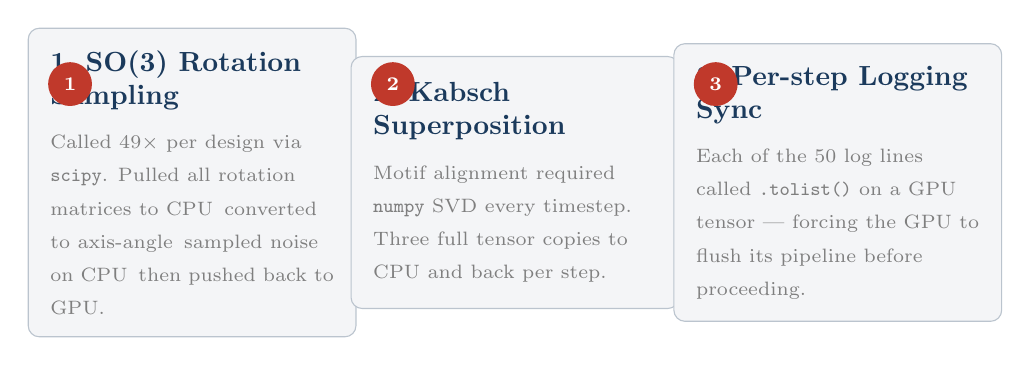
\begin{tikzpicture}
  \foreach \i/\title/\body in {
    1/{SO(3) Rotation Sampling}/{Called 49$\times$ per design via \texttt{scipy}. Pulled all rotation matrices to CPU\, converted to axis-angle\, sampled noise on CPU\, then pushed back to GPU.},
    2/{Kabsch Superposition}/{Motif alignment required \texttt{numpy} SVD every timestep. Three full tensor copies to CPU and back per step.},
    3/{Per-step Logging Sync}/{Each of the 50 log lines called \texttt{.tolist()} on a GPU tensor — forcing the GPU to flush its pipeline before proceeding.}
  }{
    \node[draw=NavyBlue!30, fill=NavyBlue!5, rounded corners=4pt,
          text width=3.6cm, minimum height=3.2cm, align=flush left,
          inner sep=8pt]
      at ({(\i-1)*4.1cm}, 0) {
        \textbf{\textcolor{NavyBlue}{\i.\ \title}}\\[4pt]
        \scriptsize\color{MidGray}\body
      };
    \node[circle, fill=CPURed, text=white, font=\scriptsize\bfseries,
          minimum size=0.5cm]
      at ({(\i-1)*4.1cm - 1.55cm}, 1.25cm) {\i};
  }
\end{tikzpicture}
\end{frame}

\begin{frame}{The A100's Slow CPU Amplified the Problem}
\begin{columns}[c]
\begin{column}{0.50\textwidth}
\begin{tikzpicture}
\begin{axis}[
  xbar,
  bar width=0.6cm,
  width=6.5cm, height=5.5cm,
  xmin=0, xmax=5,
  xlabel={Single-Core Boost (GHz)},
  xlabel style={font=\small},
  symbolic y coords={EPYC 7742\\(A100), EPYC 7413\\(L40), Ryzen 5 5600\\(RTX 3060)},
  ytick=data,
  yticklabel style={align=right, font=\scriptsize},
  axis line style={NavyBlue},
  tick style={NavyBlue},
  xmajorgrids=true,
  grid style={dashed, LightBlue!50},
  nodes near coords,
  nodes near coords style={font=\scriptsize\bfseries},
]
\addplot[fill=SteelBlue!70, draw=NavyBlue] coordinates {
  ({EPYC 7742\\(A100)},   2.25)
  ({EPYC 7413\\(L40)},    3.60)
  ({Ryzen 5 5600\\(RTX 3060)}, 4.40)
};
\end{axis}
\end{tikzpicture}
\end{column}
\begin{column}{0.47\textwidth}
  \small
  The diffusion loop is \textbf{sequential Python} — single-core speed determines how fast the CPU can feed the GPU between forward passes.
  \vspace{0.5em}

  The EPYC 7742 (A100 machine) is a Zen~2 server chip optimised for \textbf{throughput across many cores}, not single-core latency.
  \vspace{0.5em}

  At 2.25~GHz, each CPU-side operation took nearly \textbf{2$\times$ longer} than on the Ryzen 5 5600 — leaving the A100 starved.
\end{column}
\end{columns}
\end{frame}

% ══════════════════════════════════════════════════════════════════════════════
%  4. SOLUTIONS
% ══════════════════════════════════════════════════════════════════════════════
\sectionslide{4. Solutions Implemented}

\begin{frame}{Four Targeted Changes — No Architecture Modifications}
\begin{tikzpicture}
  \foreach \i/\tag/\title/\body in {
    1/{\texttt{diffusion.py}}/{SO(3) Sampling Ported to GPU}/{Replaced \texttt{scipy} axis-angle conversion and \texttt{numpy} interpolation with native PyTorch ops. Noise sampled with \texttt{torch.randn} on device.},
    2/{\texttt{utils.py}}/{Kabsch Alignment Ported to GPU}/{Replaced \texttt{numpy} SVD and all three \texttt{.cpu().numpy()} calls with \texttt{torch.linalg.svd}. Result stays on GPU.},
    3/{\texttt{utils.py}}/{Device Consistency Fixed}/{Corrected tensor device mismatches in the denoising loop that were silently triggering CPU fallbacks on every timestep.},
    4/{\texttt{inference.py}}/{TF32 + Logging Sync Removed}/{Enabled TF32 matmul precision on tensor cores. Removed \texttt{.tolist()} GPU flush from per-step log.}
  }{
    \node[draw=Green!40, fill=Green!5, rounded corners=4pt,
          text width=2.9cm, minimum height=3.8cm, align=flush left,
          inner sep=7pt]
      at ({(\i-1)*3.3cm}, 0) {
        \textcolor{MidGray}{\tiny\tag}\\[2pt]
        \textbf{\textcolor{NavyBlue}{\small\title}}\\[4pt]
        \scriptsize\color{MidGray}\body
      };
    \node[circle, fill=Green, text=white, font=\scriptsize\bfseries,
          minimum size=0.5cm]
      at ({(\i-1)*3.3cm - 1.2cm}, 1.65cm) {\i};
  }
\end{tikzpicture}
\end{frame}

% ══════════════════════════════════════════════════════════════════════════════
%  5. RESULTS
% ══════════════════════════════════════════════════════════════════════════════
\sectionslide{5. Results}

\begin{frame}{1.5–2 Minutes Saved Per Design on RTX 3060}
\begin{columns}[c]
\begin{column}{0.52\textwidth}
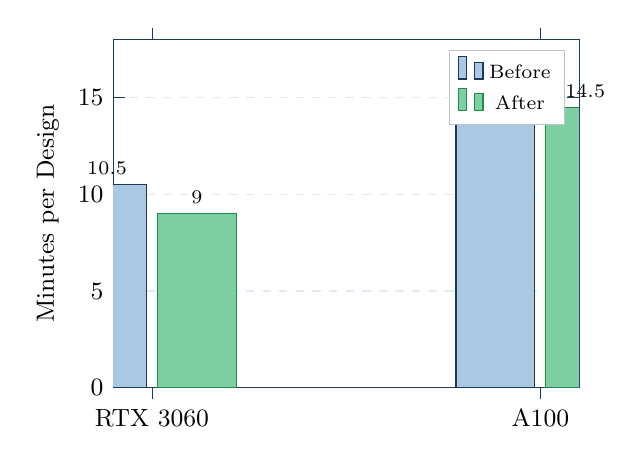
\begin{tikzpicture}
\begin{axis}[
  ybar=4pt,
  bar width=1.0cm,
  width=7.5cm, height=6cm,
  ymin=0, ymax=18,
  ylabel={Minutes per Design},
  ylabel style={font=\small},
  symbolic x coords={RTX 3060, A100},
  xtick=data,
  xticklabel style={font=\small},
  yticklabel style={font=\small},
  axis line style={NavyBlue},
  tick style={NavyBlue},
  ymajorgrids=true,
  grid style={dashed, LightBlue!50},
  legend style={at={(0.97,0.97)}, anchor=north east, font=\scriptsize,
                draw=NavyBlue!30},
  nodes near coords,
  nodes near coords style={font=\scriptsize\bfseries},
]
\addplot[fill=SteelBlue!40, draw=NavyBlue] coordinates {
  (RTX 3060, 10.5) (A100, 16)
};
\addplot[fill=Green!60, draw=Green!80!black] coordinates {
  (RTX 3060, 9.0) (A100, 14.5)
};
\legend{Before, After}
\end{axis}
\end{tikzpicture}
\end{column}
\begin{column}{0.45\textwidth}
  \begin{block}{RTX 3060}
    \small
    $10.5 \rightarrow 9.0$ min \quad \textbf{(\textcolor{Green}{$-14\%$})}\\
    GPU was the bottleneck — fully saturated. Gains came from eliminating CPU stall time between forward passes.
  \end{block}
  \vspace{0.4cm}
  \begin{block}{A100}
    \small
    $16 \rightarrow 14.5$ min \quad \textbf{(\textcolor{Green}{$-9\%$})}\\
    CPU single-core speed (2.25~GHz) remains a limiting factor. Further gains require batching.
  \end{block}
  \vspace{0.4cm}
  \small\textcolor{MidGray}{Model weights, outputs, and numerical results are unchanged.}
\end{column}
\end{columns}
\end{frame}

% ══════════════════════════════════════════════════════════════════════════════
%  6. HARDWARE LANDSCAPE
% ══════════════════════════════════════════════════════════════════════════════
\sectionslide{6. Hardware Landscape}

\begin{frame}{GPU Utilization Reveals the Real Bottleneck Per Machine}
\begin{columns}[c]
\begin{column}{0.55\textwidth}
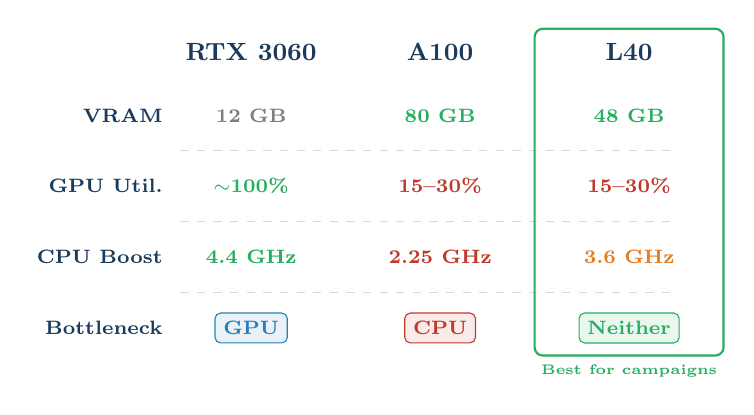
\begin{tikzpicture}
  % Column headers
  \foreach \x/\lbl in {1.8/RTX 3060, 4.2/A100, 6.6/L40}{
    \node[font=\small\bfseries, text=NavyBlue, align=center] at (\x, 3.4) {\lbl};
  }
  % Row labels
  \foreach \y/\lbl in {2.6/VRAM, 1.7/GPU Util., 0.8/CPU Boost, -0.1/Bottleneck}{
    \node[font=\scriptsize\bfseries, text=NavyBlue, anchor=east] at (0.8, \y) {\lbl};
  }
  % VRAM row
  \foreach \x/\val/\col in {1.8/12 GB/MidGray, 4.2/80 GB/Green, 6.6/48 GB/Green}{
    \node[font=\scriptsize\bfseries, text=\col] at (\x, 2.6) {\val};
  }
  % GPU Util row
  \foreach \x/\val/\col in {1.8/$\sim$100\%/Green, 4.2/15--30\%/CPURed, 6.6/15--30\%/CPURed}{
    \node[font=\scriptsize\bfseries, text=\col] at (\x, 1.7) {\val};
  }
  % CPU Boost row
  \foreach \x/\val/\col in {1.8/4.4 GHz/Green, 4.2/2.25 GHz/CPURed, 6.6/3.6 GHz/Amber}{
    \node[font=\scriptsize\bfseries, text=\col] at (\x, 0.8) {\val};
  }
  % Bottleneck row
  \foreach \x/\val/\col in {1.8/GPU/GPUBlue, 4.2/CPU/CPURed, 6.6/Neither/Green}{
    \node[draw=\col, fill=\col!10, rounded corners=2pt,
          font=\scriptsize\bfseries, text=\col, inner sep=3pt]
      at (\x, -0.1) {\val};
  }
  % Grid lines
  \foreach \y in {2.15, 1.25, 0.35}{
    \draw[MidGray!30, dashed] (0.9, \y) -- (7.2, \y);
  }
  % Highlight L40
  \draw[Green, thick, rounded corners=3pt]
    (5.4, -0.45) rectangle (7.8, 3.7);
  \node[Green, font=\tiny\bfseries] at (6.6, -0.65) {Best for campaigns};
\end{tikzpicture}
\end{column}
\begin{column}{0.42\textwidth}
  \small
  The RTX~3060 is \textbf{accidentally efficient} at $B{=}1$: its modest GPU is fully saturated by one design at a time.
  \vspace{0.5em}

  The A100 and L40 are \textbf{underutilised} at $B{=}1$ — they are designed for large parallel workloads.
  \vspace{0.5em}

  The L40 has the best combination: a faster server CPU (Zen~3) and 48~GB VRAM — \textbf{enough room to batch multiple designs in one forward pass}.
\end{column}
\end{columns}
\end{frame}

% ══════════════════════════════════════════════════════════════════════════════
%  7. FUTURE WORK
% ══════════════════════════════════════════════════════════════════════════════
\sectionslide{7. Future Work}

\begin{frame}{Batching Would Unlock the Full Potential of the L40 and A100}
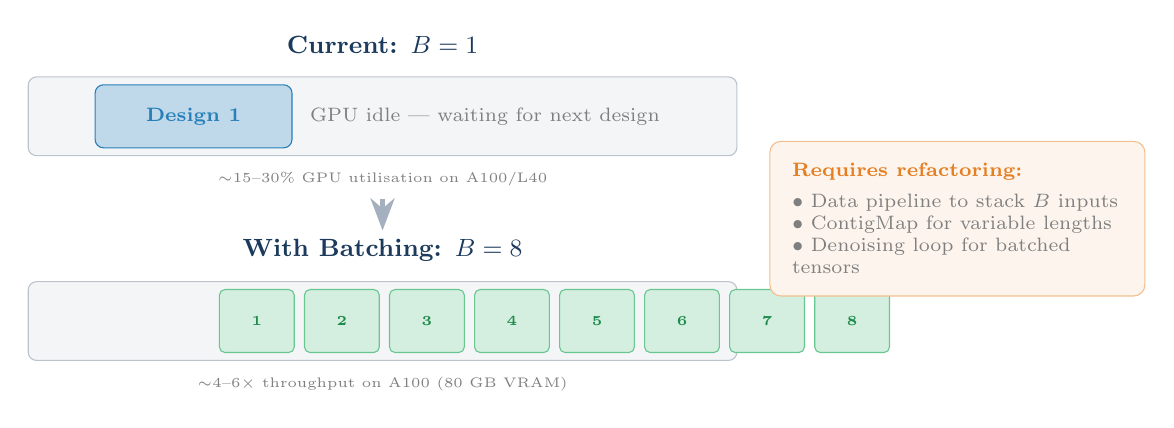
\begin{tikzpicture}

% ── B=1 ───────────────────────────────────────────────────────────────────────
\node[font=\small\bfseries, text=NavyBlue] at (1.5, 2.8) {Current: $B=1$};

\node[draw=NavyBlue!30, fill=NavyBlue!5, rounded corners=3pt,
      minimum width=9.0cm, minimum height=1.0cm] at (1.5, 1.9) {};
\node[draw=GPUBlue, fill=GPUBlue!30, rounded corners=3pt,
      minimum width=2.5cm, minimum height=0.8cm,
      font=\scriptsize\bfseries, text=GPUBlue] at (-0.9, 1.9) {Design 1};
\node[font=\scriptsize, text=MidGray] at (2.8, 1.9) {GPU idle \textemdash\ waiting for next design};
\node[MidGray, font=\tiny] at (1.5, 1.1) {$\sim$15--30\% GPU utilisation on A100/L40};

% ── B=8 ───────────────────────────────────────────────────────────────────────
\node[font=\small\bfseries, text=NavyBlue] at (1.5, 0.2) {With Batching: $B=8$};

\node[draw=NavyBlue!30, fill=NavyBlue!5, rounded corners=3pt,
      minimum width=9.0cm, minimum height=1.0cm] at (1.5, -0.7) {};
\foreach \i in {1,...,8}{
  \node[draw=Green!70, fill=Green!20, rounded corners=2pt,
        minimum width=0.95cm, minimum height=0.8cm,
        font=\tiny\bfseries, text=Green!80!black]
    at ({-2.75 + (\i-1)*1.08cm}, -0.7) {\i};
}
\node[MidGray, font=\tiny] at (1.5, -1.5) {$\sim$4--6$\times$ throughput on A100 (80~GB VRAM)};

% ── Arrow ─────────────────────────────────────────────────────────────────────
\draw[-{Stealth[scale=1.2]}, NavyBlue!40, line width=1.5pt]
  (1.5, 0.85) -- (1.5, 0.45);

% ── Side note ─────────────────────────────────────────────────────────────────
\node[draw=Amber!50, fill=Amber!8, rounded corners=4pt,
      text width=4.2cm, align=flush left, inner sep=8pt,
      font=\scriptsize]
  at (8.8, 0.6) {
    \textbf{\textcolor{Amber}{Requires refactoring:}}\\[3pt]
    \textcolor{MidGray}{%
      $\bullet$ Data pipeline to stack $B$ inputs\\
      $\bullet$ ContigMap for variable lengths\\
      $\bullet$ Denoising loop for batched tensors%
    }
  };

\end{tikzpicture}
\end{frame}

\begin{frame}{Roadmap}
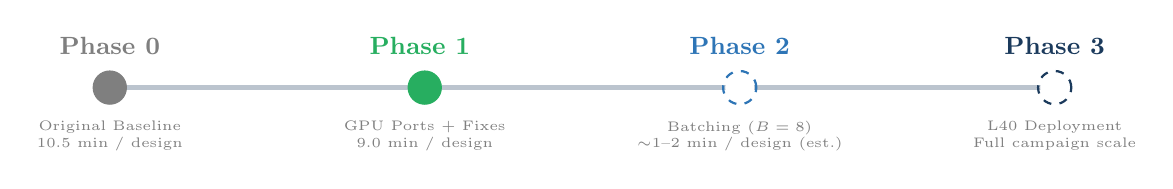
\begin{tikzpicture}
  % Timeline line
  \draw[NavyBlue!30, line width=2pt] (0, 0) -- (12, 0);

  % Milestones
  \foreach \x/\label/\sublabel/\col/\done in {
    0/{Phase 0}/{Original Baseline\\10.5 min / design}/MidGray/1,
    4/{Phase 1 \checkmark}/{GPU Ports + Fixes\\9.0 min / design}/Green/1,
    8/{Phase 2}/{Batching ($B=8$)\\$\sim$1--2 min / design (est.)}/SteelBlue/0,
    12/{Phase 3}/{L40 Deployment\\Full campaign scale}/NavyBlue/0
  }{
    \ifnum\done=1
      \filldraw[\col] (\x, 0) circle (6pt);
    \else
      \draw[\col, dashed, thick] (\x, 0) circle (6pt);
      \filldraw[white] (\x, 0) circle (5pt);
    \fi
    \node[font=\small\bfseries, text=\col, align=center, above=0.3cm] at (\x, 0)
      {\label};
    \node[font=\tiny, text=MidGray, align=center, below=0.3cm] at (\x, 0)
      {\sublabel};
  }
\end{tikzpicture}
\end{frame}

% ══════════════════════════════════════════════════════════════════════════════
%  SUMMARY
% ══════════════════════════════════════════════════════════════════════════════
\begin{frame}{Summary}
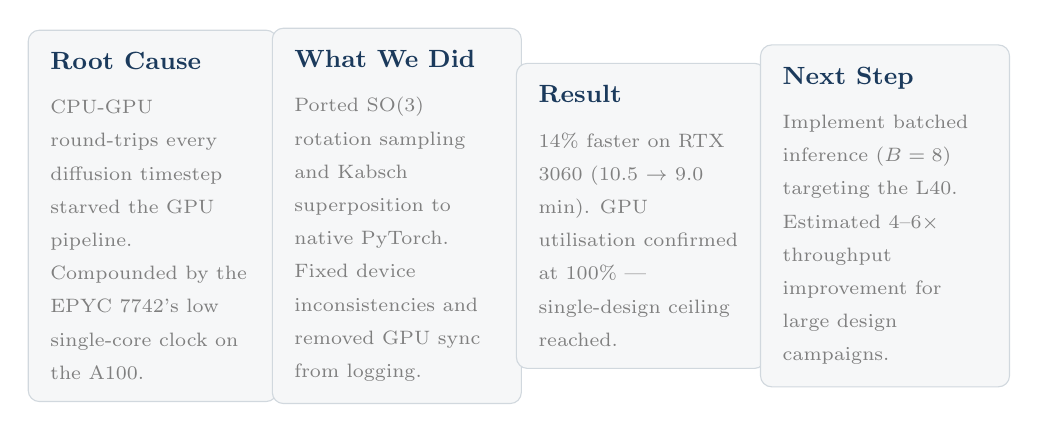
\begin{tikzpicture}
  \foreach \i/\emoji/\title/\body in {
    1/{$\triangleright$}/{Root Cause}/{CPU-GPU round-trips every diffusion timestep starved the GPU pipeline. Compounded by the EPYC 7742's low single-core clock on the A100.},
    2/{$\triangleright$}/{What We Did}/{Ported SO(3) rotation sampling and Kabsch superposition to native PyTorch. Fixed device inconsistencies and removed GPU sync from logging.},
    3/{$\triangleright$}/{Result}/{14\% faster on RTX 3060 (10.5 $\to$ 9.0 min). GPU utilisation confirmed at 100\% — single-design ceiling reached.},
    4/{$\triangleright$}/{Next Step}/{Implement batched inference ($B=8$) targeting the L40. Estimated 4--6$\times$ throughput improvement for large design campaigns.}
  }{
    \node[draw=NavyBlue!20, fill=NavyBlue!4, rounded corners=4pt,
          text width=2.6cm, minimum height=3.0cm, align=flush left,
          inner sep=8pt]
      at ({(\i-1)*3.1cm}, 0) {
        \textbf{\textcolor{NavyBlue}{\small\title}}\\[4pt]
        \scriptsize\color{MidGray}\body
      };
  }
\end{tikzpicture}
\end{frame}

% ── Thank you ─────────────────────────────────────────────────────────────────
\begin{frame}[plain]
\begin{tikzpicture}[remember picture, overlay]
  \fill[NavyBlue] (current page.south west) rectangle (current page.north east);
  \node[white, font=\LARGE\bfseries] at (current page.center) {Thank You};
  \node[LightBlue, font=\normalsize, below=0.6cm of current page.center]
    {Questions?};
\end{tikzpicture}
\end{frame}

\end{document}
